\section{Architecture}
In order to provide users with all the requested functionality, the team was in need for something more than a Android application. We also needed a back-end in order to provide statistical data and to collect data from users home.

The implementation consisted of three parts. The server, the device in the users home used to collect and send usage data, and the Android application.

\subsection{Server}
The server consisted of two parts. One for handling requests from the Android application and one for storing data that is collected in the users home. 
The part that handles the Android application runs Dropwizard~\cite{dropwizard}, which is a collection of Java libraries that together constitutes a REST service. 

These libraries include Jetty~\cite{jetty}, Jersey~\cite{jersey}, JDBC~\cite{jdbc}, and Jackson~\cite{jackson} and are discussed in further detail in \todo{\textbf{Add: }section}.
The server exposed a set of URLs that provided the Android application with 
possibilities to get and store data from the database. The other part, that stores data from the users home is under development.

\subsection{Android Application}
The application runs on the users' Android device was designed to run on Android version 4.0 or greater. As of March 2014 this includes 79,7\% of Android devices~\cite{AndroidDeviceFragmentation}. The rest is on the old Android version 2.3 and above. The team decided not to include these devices since the application is a proof-of-concept, and for the purposes of the app, the team assumed that the relevant users would have a relatively modern phone. 

The architecture heavily relied on using ContentProviders~\cite{contentproviders} for database access. This gave a uniform access model for the data, that would not run on the UI thread. When lists of data is accessed for an Activity or a Fragment, then LoaderManagers~\cite{loadermanager} was used. This would handle the lifcecycle of data change notification through the cursor. 

The remaining problem is where to place the business logic for data manipulation. This is where the pattern Model-View-Presenter (MVP)~\cite{mvp} comes in. MVP is a Model-View-Controller (MVC)~\cite{mvc} derivative. All business logic is handled in presenter classes. Through this uniform access, all logic applied to data preservation (sever syncronization), and data control can be done. The lifecycle of the presenter classes is in the base Activity class, and all other sub fragments can get access to it though a interface. This pushes almost all logic into the presenters, making the fragments code clean.

The application will follow standard Android design guidelines~\cite{Androidgui}
when it comes to user interface design.

\subsection{Home Data Aggregator}
This device collected data from sources in the user's home. The reason why we chose this external box as opposed to using the user's phone to collect data, was that with this solution the system could fetch data at regular intervals throughout 
the whole day. This would result in that the user would not need to be home in order for the application to collect 
usage data. The device would pass data along to the external server at request from the server.

\begin{figure}[H]
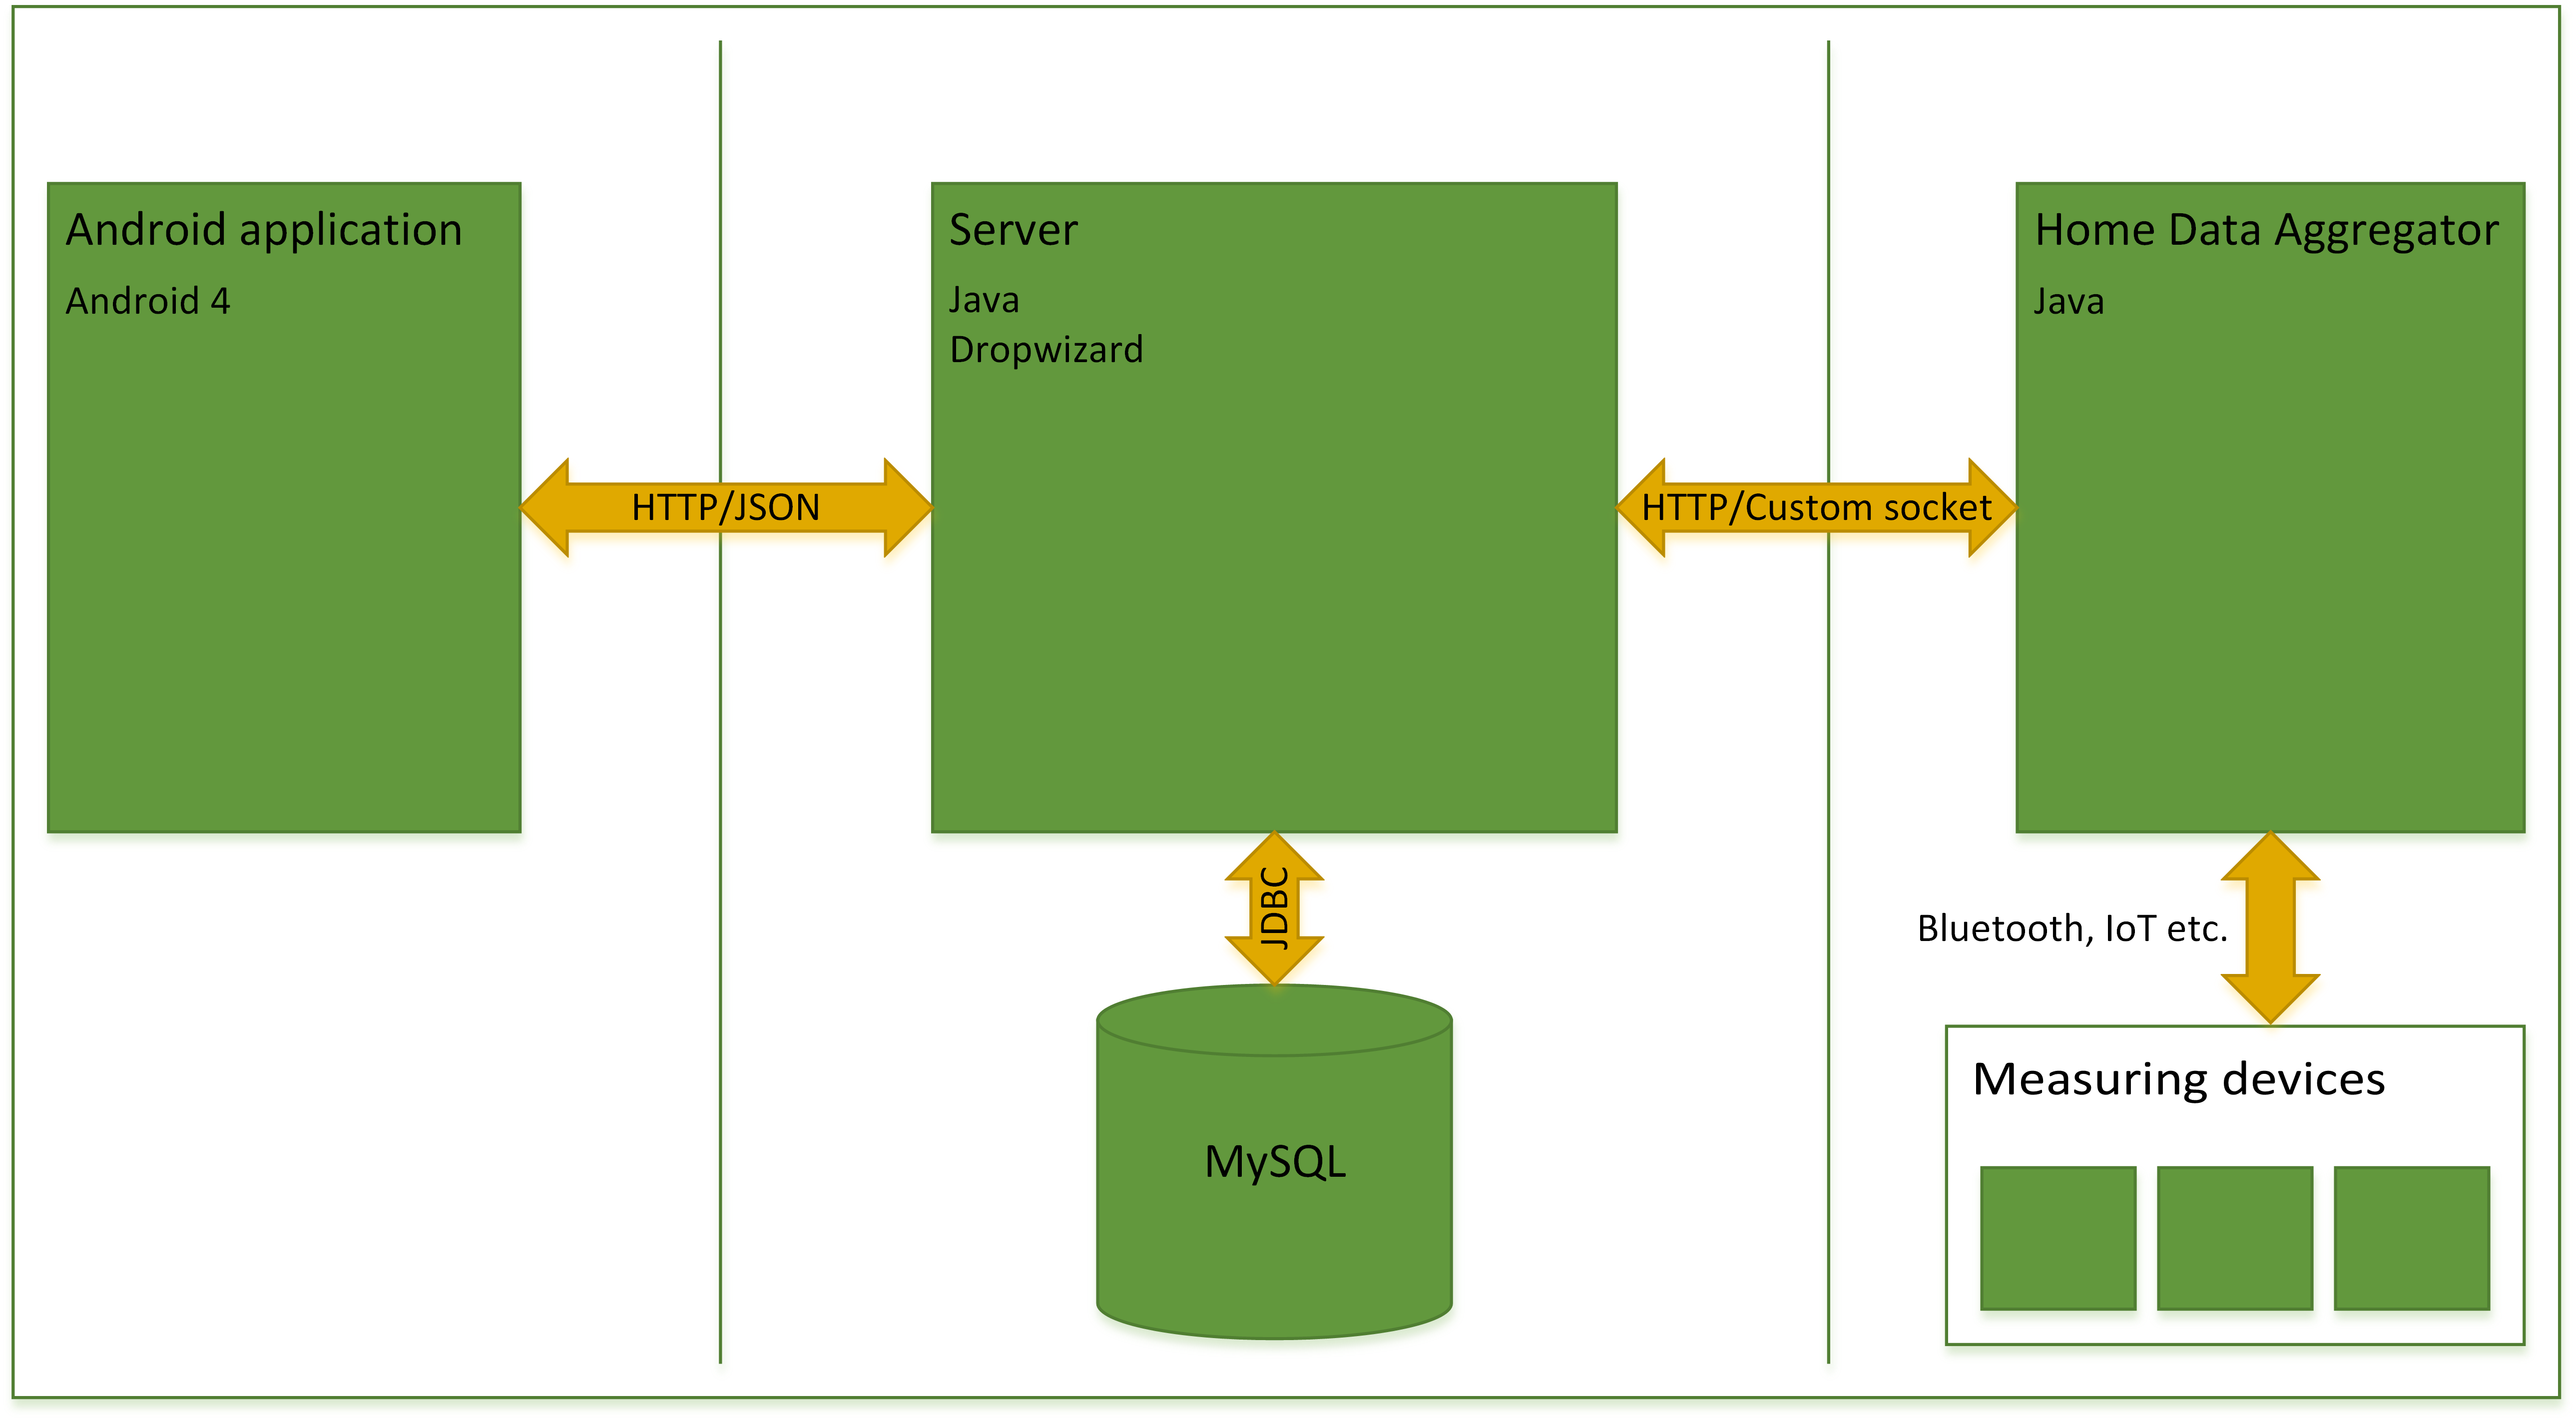
\includegraphics[width=\textwidth]{ch/implementation/fig/architecture.png}
\caption{Architecture overview}
\end{figure}